\section{Attacco all'autenticazione delle reti 5G}
In questa sezione verranno trattate le problematiche riguardo un attacco di tipo \textit{Denial of Service} all'autenticazione delle reti 5G.
Questa generazione ha risolto alcune delle probematiche legate all'autenticazione, come per esempio a differenza del 4G (LTE) l'identificatore 
dello UE viene criptato con la chiave pubblica prima di essere inviato al \textit{Core network}, evitando così di poter essere intercettato e rubato\cite{5g-vs-4g}.
Però, con il grande aumento di dispositivi connessi che questa tecnologia vuole incentivare, per esempio nel mondo dell' IOT, gli attacchi DOS saranno senz'altro più 
semplici da realizzare.\\
I SDN e NFV, componenti fondamentali per garantire le eccezionali prestazioni del 5G, potrebbero essere un efficace strumento di monitoraggio per identificare possibili 
attacchi come spiegato in \cite{dos-detection-with-sdn}.\\
Allo stesso tempo però, la centralizzazione del controllo del \textit{network} con un SDN e NFV crea le condizioni ottimali per effettuare un attacco DOS con successo\cite{5g-dos}.
\subsection{Replicazione di un attacco SIM-less}
Alla base degli attacchi trattati nella sezione 6.3 vi è la costruzione di un \textit{database} di IMSI. Questo database può essere agevolmente costruito nelle generazioni precedenti al 5G 
tramite le tecniche di IMSI \textit{catching} trattate in 6.2. Nel 5G risulta molto più difficile creare un archivio di IMSI poichè questi viaggiano in forma criptata nella rete ovvero il SUCI.

\subsection{Possibili soluzioni}
\subsubsection{Lightweight authentication}
\cite{5g-lightweight}
\subsubsection{Blockchain}
\begin{figure}[ht]
    \centering
    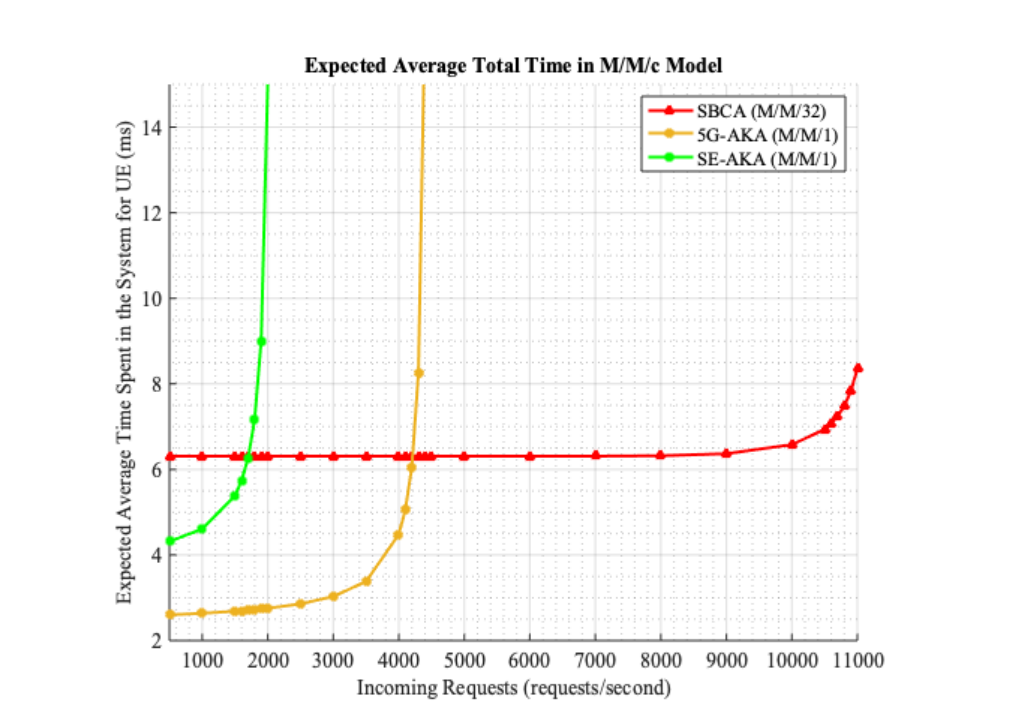
\includegraphics[width=0.8\textwidth]{images/5g-blockchain-dos.png}
    \caption{Prestazioni durante DOS della \textit{blockchain}\cite{5g-blockchain}}
\end{figure}

%Subscription Concealed Identifier
\cite{5g-imsi-encryption}
